% ============================================================================
% Title:        Brief history
% Author:       Nathaniel Thomas
% Affiliation:  Texas A&M University, Department of Nuclear Engineering
% Email:        nathaniel@tamu.edu
% Date Created: 3/11/2026
% Version:      1.0
%
% Description:
%   A .tex source file describing a brief history of the FLiNaK purifier at
%   Texas A&M University
%
% =============================================================================

\subsection{A brief history}

The project began in [INSERT DATE]
% 2021 % TODO: Confirm this date
under the supervision of
\href{https://ners.engin.umich.edu/people/raiman-stephen/}{Dr. Steven Raiman},
who was a professor at Texas A\&M at the time (\Cref{fig: steven raiman}).  \par

The construction of the system was performed by Kyle Williams
(\Cref{fig: kyle williams}), a PhD student under Dr. Raiman with an
undergradute Chemical Engineering degree
from the University of Arkansas. In the summer of 2022, Steven Raiman left
Texas A\&M, but Kyle Williams stayed behind, joining Dr. Lin Shao's
(\Cref{fig: lin shao}) group instead. In the Fall of 2022, a junior
undergraduate
Chemical Engineering student named Nathaniel Thomas
(the author of this document) to aid in the construction and operation of the
FLiNaK purifier. \par

Nathaniel Thomas contributed to setting up the HF detection for the FLiNaK
purifier, and also aided in general maintenance efforts during his time as
an undergraduate researcher. \par

\begin{figure}
  \centering
  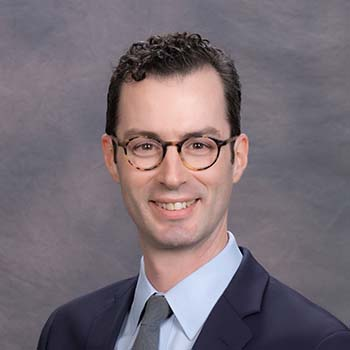
\includegraphics[width=0.2\textwidth]{./assets/pictures/steven raiman.jpg}
  \caption{An image of Dr. Steven Raiman, taken from
  \href{https://ners.engin.umich.edu/people/raiman-stephen/}{ners.engin.umich.edu}}
  \label{fig: steven raiman}
\end{figure}

\begin{figure}
  \centering
  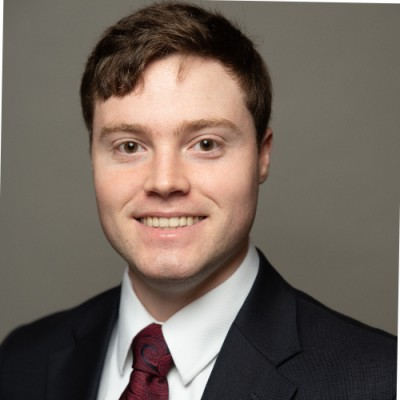
\includegraphics[width=0.2\textwidth]{./assets/pictures/kyle williams.jpeg}
  \caption{An image of Kyle Williams, taken from
  \href{https://www.linkedin.com/in/kyle-williams-443656138/}{linkedin.com}}
  \label{fig: kyle williams}
\end{figure}

\begin{figure}
  \centering
  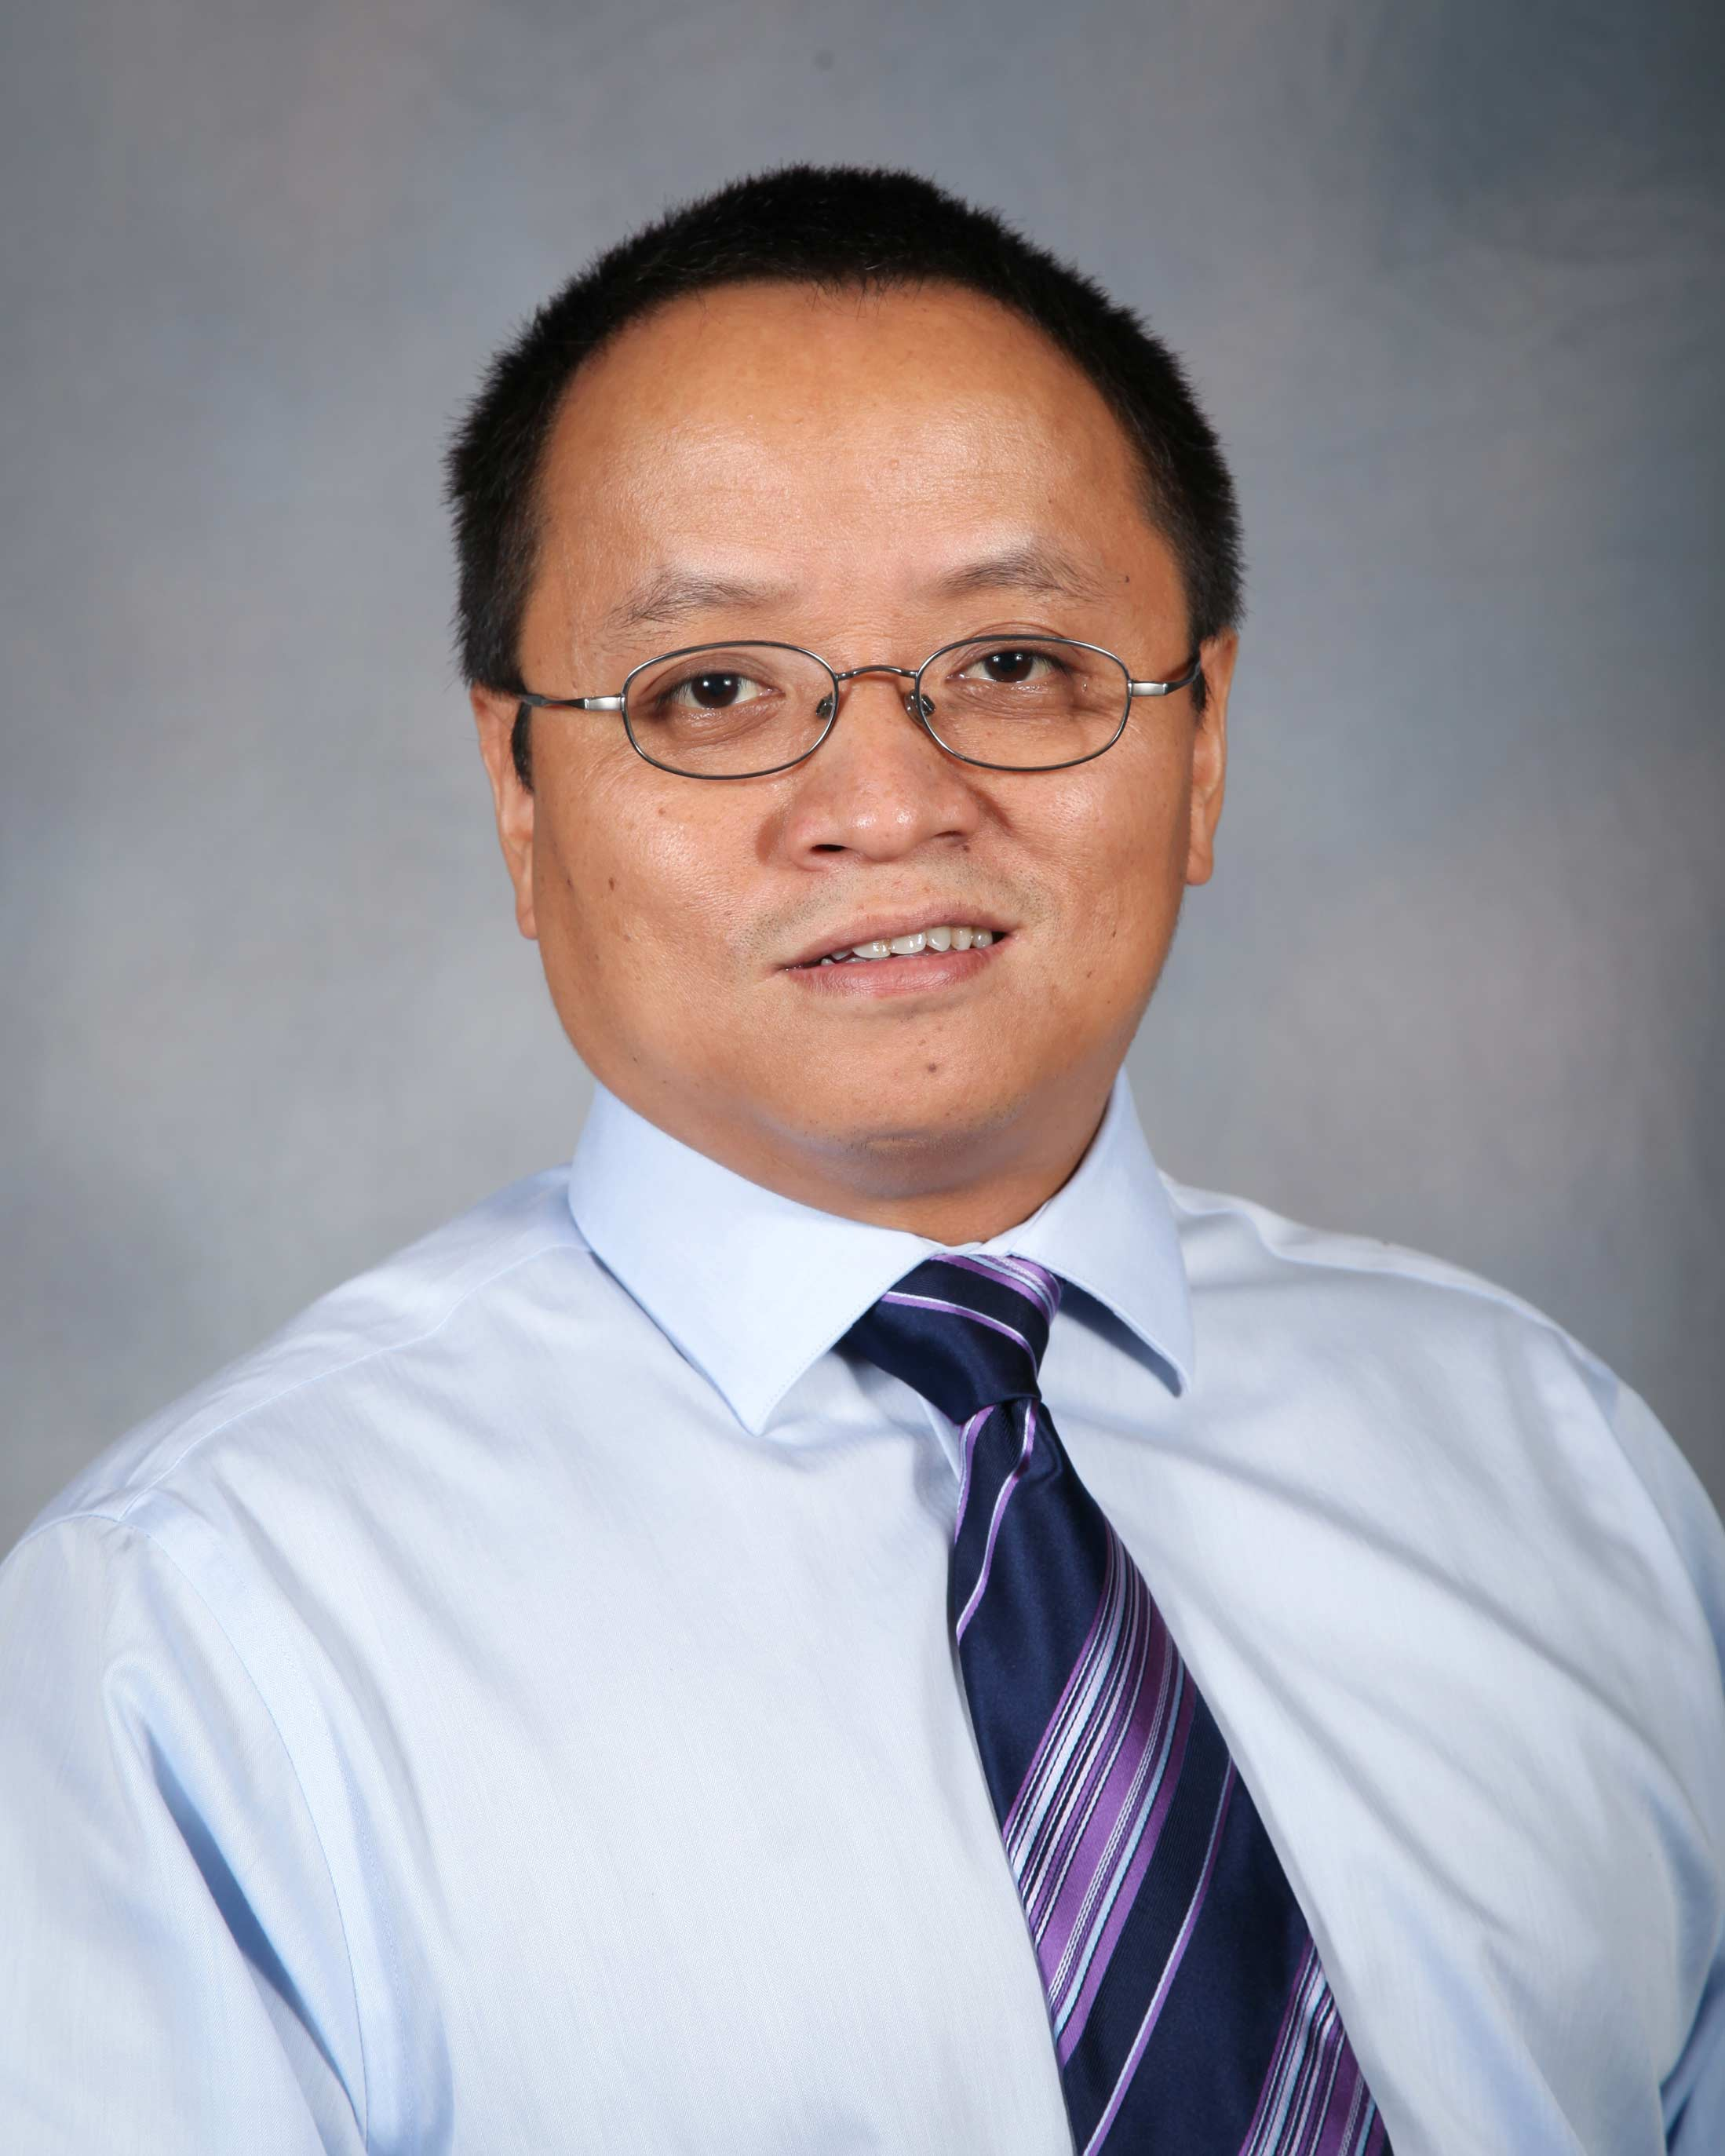
\includegraphics[width=0.2\textwidth]{./assets/pictures/lin shao.jpg}
  \caption{An image of Lin Shao, taken from
  \href{https://engineering.tamu.edu/nuclear/profiles/shao-lin.html}{engineering.tamu.edu}}
  \label{fig: lin shao}
\end{figure}

The FLiNaK purifier was run [number of times], with various issues preventing
full and proper function. While there were several runs that were
at least partially successful (refer to \Cref{sec: successful runs}),
there were many failures as well. One of the first failures was an
accidental ingress
of scrubber solution, contaminating FLiNaK with caustic base solution.
Further one, there were problems with inadequate heating during salt transfer
following purification, resulting in clogs and partial disassembly. Finally,
a major failure occured, resulting in the splillage of molten FLINaK, and
which required a complete rebuild of the purifier. The details of the
failures of the purifier are covered in \Cref{sec: failure report}. \par

% TODO: Go over this with Kyle to confirm that the history is correct.

% TODO: Elaborate
